\subsubsection{Datenformat der Audiodaten}
\label{sec:Dataformat}

Nachfolgend wird zuerst dargestellt, wie der Datenfluss vom und zum Codec aussieht und zu interpretieren bzw. verarbeiten ist. 
Sowohl der STM32 als auch der Codec unterstützen weitere Betriebsmodi (Left/Right Justified, MSB/LSB First). Hier ist nur die implementierte Variante beschrieben.

Die Abbildung \ref{pic:I2S_Datastream} zeigt einen Datenfluss, wie er aus dem Codec über die \texttt{I2S\_DOUT} Leitung heraus kommt. 
Das verwendete Datenformat ist \textit{16 Bit Data Word on a 32 Bit Frame}. Das bedeutet, dass der Samplingwert 16 Bit gross (\texttt{int16\_t}) ist, und von 16 weiteren Leerbits begleitet wird.
Der Datenfluss ist \textit{Left Justified}, was bedeutet, dass pro Abtastwert immer zuerst der linke Kanal gefolgt vom rechten Kanal übertragen wird.

\begin{figure}[H]
	\centering
	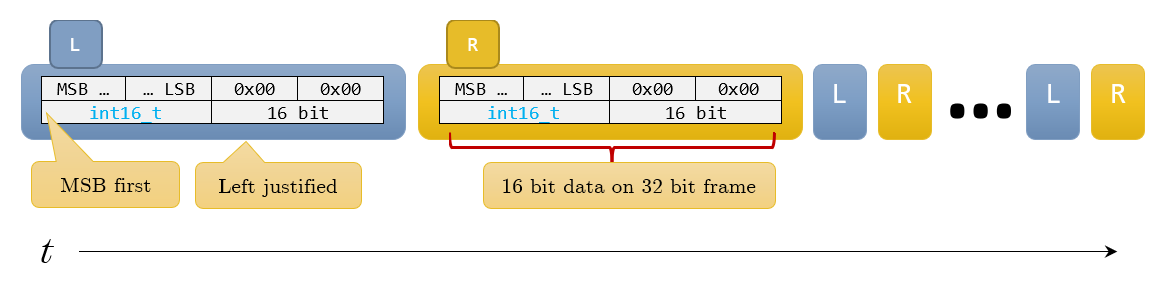
\includegraphics[width=1.0\linewidth]{I2S_Datastream}
	\caption{Zeitliche Abfolge der Samplingwerte vom und zum Codec}
	\label{pic:I2S_Datastream}
\end{figure}

Damit der Datenstrom richtig empfangen wird, ist die I\textsuperscript{2}S Schnittstelle entsprechend Konfiguriert, siehe Abschnitt \ref{sec:CubeMXI2S}.
Um die Daten automatisch im RAM des STM32F412 abzuspeichern, kommt der DMA Controller zum Einsatz, dessen Konfiguration in Abschnitt \ref{sec:CubeMXDMA} beschrieben ist.

\begin{figure}[H]
	\centering
	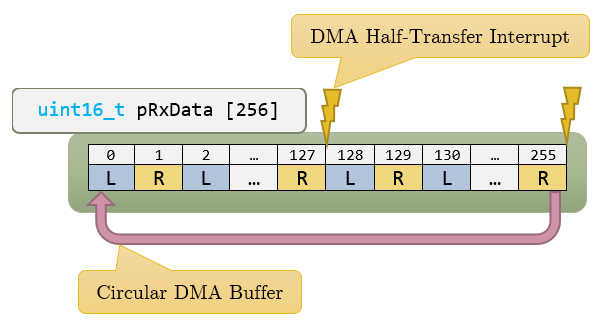
\includegraphics[width=0.6\linewidth]{DMA_CircularBuffer}
	\caption{Aufbau des Circular Buffers der beim DMA verwendet wird.}
	\label{pic:DMA_CircularBuffer}
\end{figure}

Der DMA Controller schreibt die Daten kontinuierlich in ein \texttt{uint16\_t} Array der Länge 256. Im \textit{Circular Buffer} Modus, wird beim Erreichen des Bufferende der DMA Pointer automatisch wieder an den Anfang gesetzt, siehe Abbildung \ref{pic:DMA_CircularBuffer}.
Mit der passenden Interrupt Konfiguration wird immer bei halbem und vollem Füllstand des Buffers ein \textit{DMA Half-Transfer Interrupt} ausgelöst.
So kann jeweils die Hälfte des zuvor geschriebenen Buffers verarbeitet werden.



